\section{The geometric reduction}
\label{sec:geometry}

We use the disk assertion only to compress a finite collection of surfaces.
The following restricted version of its disk conclusion is therefore sufficient.
All manifolds in the constructions before that application are smooth and
oriented; corners are rounded when necessary.
The output will be a fixed disk problem with algebraic duals, together
with a description of the cut manifolds that its hypothetical embedded
solutions would produce. The marked boundary words and their based paths
are chosen as part of the initial disk problem.

\begin{assumption}[Universal framed disk replacement]
\label{ass:disk}
Let \(M\) be a compact connected oriented smooth four-manifold with boundary.
Suppose that a finite collection of proper generic immersions
\[
 f_i\colon(D^2,S^1)\longrightarrow(M,\partial M),\qquad 1\leq i\leq k,
\]
has pairwise disjoint embedded boundary circles, and admits generically immersed
framed spheres \(g_1,\ldots,g_k\) such that
\[
 \lambda(f_i,g_j)=\delta_{ij},\qquad
 \lambda(g_i,g_j)=0,\qquad
 \widetilde\mu(g_i)=0
 \quad\text{for all }i,j.
\]
Here intersections are counted in \(\mathbb Z[\pi_1M]\), with fixed whiskers,
the diagonal equations are included, and
\[
 \widetilde\mu(g_i)\in
 \mathbb Z[\pi_1M]\big/
 \big\langle h-h^{-1},\,\mathbb Z\cdot1\big\rangle
\]
uses the additive quotient. Then the \(f_i\) can be replaced by pairwise disjoint
locally flat embedded disks with the same boundary maps and the same induced
normal framings on those boundary circles.
\end{assumption}

No relative homotopy class for the replacement disks is prescribed in
Assumption~\ref{ass:disk}. Nor does it require output dual spheres. The
unrestricted version of \cite[Theorem~A]{PRT2025} would imply this assumption,
including its framing clause. We will contradict the assumption itself.
The capped-surface contractions used below are the usual one-sided
contractions; see \cite[\S1.2]{KQ2000} and
\cite[Lemma~3.4 and its preceding discussion]{PRT2025}.
The relation between grope trees and commutator words is also used in
\cite{FK2016,FK2020}. We give the particular finite construction needed here.

\subsection{A finite list of relations}

Our commutator convention is \([a,b]=aba^{-1}b^{-1}\).
A word \(R\) in three free generators \(X_1,X_2,X_3\) will be called a
\emph{three-slot grope word} if it is the boundary word of the rooted surface
tree consisting of a punctured torus with a single tip on its first branch
and a second punctured torus on its other branch. Paths to its three tips
are part of its marking. Changing those paths inside the body can conjugate
a tip by words in the three based tips, and can conjugate the inner
commutator by such a word. Overall conjugation of the boundary word is
irrelevant to its being a relation. In particular,
\begin{equation}
\label{eq:grope-word-properties}
 \left.R\right|_{X_a=1}=1\quad(a=1,2,3),
 \qquad
 R\equiv[X_1,[X_2,X_3]]
       \pmod{\Gamma_4F(X_1,X_2,X_3)}.
\end{equation}
Here \(\Gamma_rF\) denotes the lower central series of the free group \(F\).
The first property is the \emph{Brunnian property in the three slots}:
setting any one input equal to the identity trivializes the word.
The orientations of the two surfaces can be fixed to give the displayed
sign. Indeed a tip conjugation changes its image modulo \(\Gamma_2\)
by zero, and hence changes this weight-three commutator only modulo
\(\Gamma_4\). The first assertion follows directly by deleting a branch
of the rooted tree. Equivalently, in the completed free associative algebra
over \(\mathbb Q\),
\begin{equation}
\label{eq:grope-word-leading}
 \log R(e^{Z_1},e^{Z_2},e^{Z_3})
   =[Z_1,[Z_2,Z_3]]+\text{terms of total degree at least four};
\end{equation}
each term contains a letter from every slot. These two properties,
rather than a claim that an entire vertex group is nilpotent, will be used.

Fix \(m\geq5\) and \(p\geq9\). Each plumbing block will have \(2m\)
solid-torus boundary regions, called \emph{ports}, through which it
joins other blocks. Removing these regions leaves \(2m\) boundary
tori. Write \(x_1,\ldots,x_{2m}\) for their meridians and
\(l_1,\ldots,l_p\) for the extra one-handle generators, and put
\[
 \mathcal C=\{1,l_1,\ldots,l_p\}.
\]
Before making any cut, install one marked grope body for every ordered
triple of distinct port indices, every independent choice
\(c_1,c_2,c_3\in\mathcal C\), and every independent choice
\(\delta_1,\delta_2,\delta_3\in\{1,-1\}\). Its three based tips represent
\begin{equation}
\label{eq:three-slot-inputs}
 X_a=c_a x_{r_a}^{\delta_a}c_a^{-1},
 \qquad a=1,2,3.
\end{equation}
There are at most
\[
 8(2m)(2m-1)(2m-2)(p+1)^3
\]
such bodies. Any additional fixed finite list of words in the extra letters
could be included in \(\mathcal C\) by the same construction.
In particular, neither the list of bodies nor their markings depends on
the slopes selected by the cuts below.

\begin{proposition}[Geometric reduction]
\label{prop:geometric-reduction}
For the integers \(m,p\) and the finite list just specified, there is a
compact connected oriented smooth four-manifold \(X\), constructed without
Assumption~\ref{ass:disk}, with the following properties.

It has a regular cover with deck group \(F_m\), whose block graph is the
Cayley tree of \(F_m\). Each block is a four-dimensional one-handlebody on
the \(p\) extra letters. Its exposed boundary piece is
\[
 K_v\cong
 \bigl(\#^p(S^1\times S^2)\bigr)
 \setminus\operatorname{int}\nu(L_{2m}),
\]
where \(L_{2m}\) is a \(2m\)-component unlink in a ball. The port meridians
and the extra letters freely generate \(\pi_1K_v\).
At every join, the meridian on one side is the longitude on the other.
There is a finite family of framed grope bodies with boundary in these
pieces, equivariant in the cover, realizing the list
\eqref{eq:three-slot-inputs}.

If Assumption~\ref{ass:disk} holds, there are equivariant cuts, with compact
quotient, having connected vertex pieces \(V_v\) and connected edge
three-manifolds \(Y_e\). Each \(Y_e\) has as its entire boundary the prescribed
join torus. Every corresponding three-slot grope word is trivial in
\(\pi_1V_v\).

In the index-two parity quotient, these cuts give two connected vertex
pieces \(A,B\) and \(2m\) connected oriented edge pieces \(Y_1,\ldots,Y_{2m}\).
Their ambient manifold \(X_2\) is homotopy equivalent to the graph with two
vertices and \(2m\) edges, with \(p\) additional circles at each vertex.
For any characteristic-zero field \(k\), difference of restrictions gives
\begin{equation}
\label{eq:geometry-mv-degree-two}
 H^2(A;k)\oplus H^2(B;k)
       \xrightarrow{\;\cong\;}
       \bigoplus_{i=1}^{2m}H^2(Y_i;k).
\end{equation}
In degree one it is surjective, and restricts to an isomorphism on the
kernel of evaluation on the \(p\) extra loops at each vertex.

At each boundary torus choose the two original coordinate loops
\(\alpha_i,\beta_i\) so that \(\alpha_i\) has nonzero image in
\(H_1(Y_i;k)\) and \(\beta_i\) has zero image. Such a choice is possible:
one of the original coordinate directions, not just an arbitrary slope,
is killed. Call the endpoint where \(\beta_i\) is a longitude the
\emph{plus endpoint}; there \(\alpha_i\) is the port meridian.
There are exactly \(m\) edges with plus endpoint \(A\).
After numbering these as \(1,\ldots,m\), the finite relation list includes,
at \(A\), all the required three-slot relations on any three distinct
\(\alpha_i\), and, at \(B\), those on the corresponding \(\beta_i\),
with independent conjugations by \(\mathcal C\).
\end{proposition}

The proof constructs a particular exterior \(E\) and a finite disk
family in it before making any cut. A simultaneous framed replacement
of that family alone implies all the cut conclusions of the proposition;
the universal Assumption~\ref{ass:disk} is used only to provide that
replacement. Lemma~\ref{lem:exterior-duals} specifies the fixed family
and verifies its algebraic duals. This local implication will give the
fixed counterexample in Theorem~\ref{thm:main}.

\subsection{The plumbing blocks}
\label{subsec:plumbing-blocks}

Start with a standard four-dimensional one-handlebody with \(2m+p\)
one-handles. Attach a cancelling two-handle to each of the first \(2m\)
one-handles, using the product framing and disjoint standard attaching
regions. Before plumbing, the resulting block \(B\) is a one-handlebody
on the remaining \(p\) handles. The belt circles of the cancelling
two-handles are a standard unlink in a ball in \(\partial B\).
One can see each component separately from the cancelling pair:
the complement of its attaching solid torus in \(S^1\times S^2\) is a
solid torus, which becomes the complement of the belt unknot after
cancellation. The framed attaching pushoff is its belt meridian.
The cancellation regions for different pairs are disjoint.

Pair the \(2m\) two-handles. In each handle choose a small product patch
\(D^2_{\mathrm{base}}\times D^2_{\mathrm{fibre}}\), and plumb the patches
of its pair by interchanging the two factors. This is mutual plumbing;
there are no self-plumbings. To specify the local manifold structure,
the two branches at a plumbing can be represented by
\[
 \bigl(D^2_R\times D^2_r\bigr)
 \ \cup\
 \bigl(D^2_r\times D^2_R\bigr)
 \subset\mathbb R^2\times\mathbb R^2,\qquad 0<r<R.
\]
Their overlap is the product ball \(D^2_r\times D^2_r\). Rounding its
corners gives the usual smooth plumbing chart. Distinct patches are
disjoint. The factor interchange preserves the orientation in dimension
four, and the product framings fix the signs of the resulting transverse
core intersections.

Equivalently, take one copy \(B_v\) for each vertex of the Cayley tree of
\(F_m=\langle a_1,\ldots,a_m\rangle\), and identify the designated patches
of \(B_v\) and \(B_{va_j}\) by this chart. Neighbouring blocks intersect in
one product ball, and there are no other or triple intersections.
Left translation acts freely. The quotient is the finite plumbing \(X\),
and the union is its regular cover \(\widetilde X\).
Since all attaching intersections are contractible cofibrations, the
homotopy type of the union is obtained by joining the block homotopy
types along the tree. Thus
\begin{equation}
\label{eq:plumbing-homotopy}
 \widetilde X\simeq
 \text{the Cayley tree with \(p\) circles attached at each vertex}.
\end{equation}
This is not an assertion that \(\widetilde X\) is the universal cover:
the extra circles remain.

At a product patch the removed part of the unplumbed block boundary is a
solid-torus neighbourhood of the belt circle. Its boundary is
\(S^1_{\mathrm{base}}\times S^1_{\mathrm{fibre}}\).
Consequently the exposed boundary is exactly the piece \(K_v\) in
Proposition~\ref{prop:geometric-reduction}, with a torus collar at each join.
The factor interchange exchanges the two peripheral slopes.
An unlink longitude bounds a disk in \(K_v\), whereas its meridian is
one of its free generators. Adding the \(p\) extra one-handles gives the
remaining free generators \(l_s\).

Fix boundary whiskers for these generators. In the cover, fix the boundary
map to the tree which is constant on each \(K_v\) core and crosses the
corresponding tree edge on every torus collar. The middle of each collar
maps to the midpoint of that edge. The construction is equivariant.
It descends both to the one-vertex graph and to the parity quotient.

\subsection{Marked grope bodies and their framings}

The plumbing fixes the port meridians and peripheral slopes. We next
place the finite list of surface bodies with their prescribed based tip
curves, and match their framings to the handle cores. These choices must
be made before the exterior disk problem is defined.

\begin{lemma}[The marked body model]
\label{lem:marked-body}
The two-stage grope body used in \eqref{eq:grope-word-properties} has a
three-dimensional handlebody thickening which, with its three marked
tip annuli, is a boundary join of three longitudinal-annulus collars.
Finitely many copies can be placed disjointly in the boundary of the
initial one-handlebody, with prescribed parallel tip tracks to the
cancelling-handle attaching regions and with the external conjugations
\eqref{eq:three-slot-inputs}. Their surface framings can be matched to the
handle-core framings.
\end{lemma}

\begin{proof}
We first identify the thickening together with its tip annuli, then
place the finite marked family, and finally match the surface framings
to the cap framings while keeping the terminal attaching circles fixed.

\smallskip\noindent\textbf{1. Primitive tip annuli.}\quad
Thicken a punctured torus \(S\) to \(S\times[-1,1]\).
Put its two selected basis curves on opposite faces of this product.
There are disjoint proper cutting arcs in \(S\), each dual to one basis
curve and disjoint from the other. For an explicit model, puncture the
square torus near \((1/2,1/2)\), take the basis circles at \(y=1/4\)
and \(x=1/4\), and take the cutting arcs at \(x=1/2\) and \(y=1/2\),
with their ends on the puncture. The only intersection of the latter
two arcs was removed by the puncture. Their products with the interval
are disjoint meridian disks, each meeting just its own marked tip once.

For the lower stage, view the primitive \(b\)-annulus as the longitudinal
annulus of a solid torus. That solid torus is an annular collar, up to
rounding, and the rest of the lower handlebody is the spare \(a\)-handle.
Glue the annular boundary of the upper punctured-torus product to this
\(b\)-annulus. Gluing the collar only thickens that annulus on the upper
handlebody. Extend the two upper meridian disks across the collar.
Their traces occupy finitely many strips there. Place the feet and return
arc of the spare \(a\)-handle in a complementary interval. Its meridian
disk is then disjoint from both extended upper disks. We have obtained
three disjoint disk duals for the three marked tips.

This is a statement about the marked annuli, not just about a free basis.
Cut the handlebody along the three dual disks. Each marked annulus becomes
a rectangle on the boundary of the resulting ball, joining only the two
faces of its own cutting disk. The rectangles are disjoint. A neighbourhood
of each rectangle together with its two disk faces is a disk in the
boundary sphere, disjoint from the other two such disks. Smooth their
corners. A smooth isotopy of the boundary sphere carries these three
labelled disk neighbourhoods to standard ones; within each neighbourhood,
choose it also to standardize the two disk faces and their connecting
rectangle. This last choice is an isotopy of a disk containing two
subdisks joined by a band. Extend the boundary isotopy over the ball
by smooth isotopy extension. Reattaching the handles therefore identifies
the \emph{marked} smooth handlebody with a boundary join of the three
longitudinal-annulus collars.

\smallskip\noindent\textbf{2. Finite placement with based paths.}\quad
Reserve, on the attaching regions in the initial boundary, disjoint
annuli of product parallels for every tip in the finite list. Join their
thin collars by thin tubes along the desired based graph paths, avoiding
the reserved approaching strips. Finitely many arcs in a three-manifold
can be made disjoint, apart from the prescribed common ends of a graph;
parallel copies separate repeated portions. Regular neighbourhoods
therefore give the required disjoint marked handlebodies. A path winding
along an extra handle changes a based tip by the prescribed external
conjugation while leaving its free attaching curve a parallel of the
same cancelling-handle attaching loop. Paths internal to the marked
body can add only the core-word changes already allowed in
\eqref{eq:grope-word-properties}.

\smallskip\noindent\textbf{3. Matching the cap framings.}\quad
The placement fixes the external paths and the terminal product circles
at the two-handles. We now vary the winding of each surface ribbon and
its return collar to match the cap's normal framing, without moving
those terminal circles or paths. These choices precede the definition
of the exterior disk problem.

In an oriented three-dimensional body crossed with an interval, frame a
surface normal bundle by its
oriented normal in the body and the interval vector. At a tip, a cap collar
departing in the first normal direction has normal frame consisting of
the in-surface direction transverse to the tip and the interval vector.
Transport this ordered pair with the collar to the attaching region.
The discrepancy with the two-handle core's product frame is an integer.
It can be changed on the relevant solid-torus handle by
\[
 (\theta,z)\longmapsto(\theta,e^{in\theta}z),\qquad n\in\mathbb Z.
\]
The core stays fixed and the marked longitude changes by \(n\) meridians.
The three disk duals make these choices independent. To realize the
winding change with the same terminal product circle, choose the return
collar after making the twist. Use coordinates
\(S^1_\theta\times D^2_z\times[0,1]_u\) around a
separated tip and its return collar.  A twisted surface ribbon has local
form \((\theta,t e^{in\theta},0)\).  Its outgoing normal in the
three-dimensional body is \(i e^{in\theta}\).  Choose an embedded
plane arc \((a(s),b(s))\), \(0\leq s\leq1\), with
\(a(0)=a(1)=b(0)=0\), \(b(1)=1\), \(a'(0)>0\),
\(b'(0)=0\), and \(a=0\), \(b'>0\) near \(s=1\).
We may require \(b'>0\) for \(0<s\leq1\).  Then
\[
 (\theta,s)\longmapsto
       \bigl(\theta,a(s)i e^{in\theta},b(s)\bigr)
\]
is an embedded cap collar.  It leaves the ribbon in the required
outgoing direction and ends at the same product circle \(z=0,u=1\),
independently of \(n\).  In its normal quotient bundle a frame is given by
\[
 v_n=e^{in\theta},\qquad
 w_n=a'(s)\partial_u-b'(s)i e^{in\theta}.
\]
The two vectors are independent modulo the tangent plane; orthogonal
projection gives a normal frame if desired.  At the initial circle this
is the surface transverse vector together with the collar vector.  At
the terminal circle it is, up to a constant change of frame,
\((e^{in\theta},i e^{in\theta})\), whose winding relative to the
product core frame is \(n\).  Thus the framing discrepancy changes by an
arbitrary integer while the terminal cap circle stays fixed.  If a handle
foot is to remain fixed, replace \(e^{in\theta}\) by a degree-\(n\)
circle map constant near that foot.  The disjoint tip neighbourhoods
allow all these choices simultaneously.  The construction uses the
separated tip representatives on the opposite faces of the surface
products, not disjointness of the unpushed symplectic basis curves.

Choose the integers to remove the framing discrepancies. This transports
the body and its marked annuli together; it does not add a relative Euler
term to a previously fixed cap. Meridians are null in the handlebody, so
the core words and their leading commutator terms are unchanged.
The twists are fixed near the connector feet, so the external paths
realizing the \(c_a\) are unchanged.  Any internal change of path is a
word \(W(X_1,X_2,X_3)\) in the three abstract tips of the marked
handlebody.  Under the external marking
\(X_a=c_a x_{r_a}^{\delta_a}c_a^{-1}\), this word specializes to
\(W(1,1,1)=1\) when the three port meridians are trivial, even if the
extra-letter holonomies are not trivial.  Thus such path changes do not
alter the degree-three term in \eqref{eq:grope-word-leading}.

Finally put the bodies at an inner level of a short boundary collar, with
their initial boundary and three tip tracks returning to the outer level
in disjoint collars of the four marked curves. The initial boundary avoids
the attaching regions. The two directions at a symplectic pair depart on
opposite normal sides. Continue the tip tracks into separate product
parallels of the two-handle cores. These caps miss every body away from
their own attachments. Their only possible intersections are the core
intersections in the specified plumbing charts.
\end{proof}

In particular the finite family is constructed without knowing the future
cut pieces. Each cap is individually embedded: a core has no self-plumbing.
Caps of different labels may intersect, and no disjointness of their
spanning surfaces or of all their interiors is asserted.

\subsection{The disk problem in the exterior}

The marked bodies have now been placed with framed caps. Removing only
their bottom surfaces leaves an exterior in which one cap per body is
the input disk. The remaining upper stage will supply its algebraic
dual sphere; the unused upper cap will identify the group-ring labels
needed for cancellation.

Denote the disjoint bottom punctured tori by \(S_1,\ldots,S_k\).
Choose their open product tubes, including their proper boundary collars,
and put
\[
 E=X\setminus\bigcup_{j=1}^k\operatorname{int}\nu(S_j).
\]
The tubes are chosen after the finite placements of
Lemma~\ref{lem:marked-body}. They can be sufficiently thin that they avoid
all the upper caps and meet the upper bodies only in their short attaching
collars. The exterior is connected: a path can be moved off finitely many
proper codimension-two surfaces and then off their sufficiently small
tubes. It is a compact oriented smooth four-manifold after rounding.

\begin{lemma}[Algebraic duals in the exterior]
\label{lem:exterior-duals}
There are proper generically immersed disks \(f_j\) in \(E\), with
disjoint boundary circles and with the bottom-surgery framings, and framed
spheres \(g_j\) in \(E\), such that
\[
 \lambda(f_i,g_j)=\delta_{ij},\qquad
 \lambda(g_i,g_j)=0,\qquad
 \widetilde\mu(g_j)=0 .
\]
All equalities hold over \(\mathbb Z[\pi_1E]\).
\end{lemma}

\begin{proof}
Write \(D_{x,j}\) for the single cap on the \(a\)-side of \(S_j\), and use
as \(f_j\) its proper truncation on \(\partial\nu(S_j)\).
Its product framing is the framing
required for compression of the bottom.

Let \(U_j\) be the upper punctured torus. Write \(D_{y,j}\) for its chosen
surgery cap and \(D_{z,j}\) for the other cap. Compress \(U_j\) along
\(D_{y,j}\). Cutting \(U_j\) along its \(y\)-curve gives a pair of pants;
fill its two new boundary components by opposite parallel copies of
\(D_{y,j}\). The result is a disk
\begin{equation}
\label{eq:one-sided-contraction}
 C_j=U_j^{\mathrm{cut}}\cup D_{y,j}^{+}\cup(-D_{y,j}^{-})
\end{equation}
with boundary a parallel of \(b_j\). Its collar is on the outgoing side
of the upper attachment. The unused \(D_{z,j}\) is not part of \(C_j\):
it will instead give a null-homotopy in \(E\) identifying the group-ring
labels of the two surgery-cap sheets.

Take the normal-circle torus over a parallel of \(b_j\) near
\(\partial\nu(S_j)\), and compress it with two parallels of \(C_j\).
Here is a collar model fixing the relevant separations. Use coordinates
\((s,t,r,\theta)\), where \(s\) is along \(b_j\), \(t\) is transverse to it
on \(S_j\), and \((r,\theta)\) are polar coordinates normal to \(S_j\).
The torus is \(t=0,\ r=\rho\). The \(a\)-cap collar and the upper attachment
depart at distinct angles \(\theta_A,\theta_B\).
Remove the thin compression band at \(\theta_B\), keep the annulus
containing \(\theta_A\), and place the interiors of the two compression
disks outside radius \(\rho\). Thus
\begin{equation}
\label{eq:compressed-rim-sphere}
 g_j=R_j^{\mathrm{cut}}\cup C_j^+\cup(-C_j^-).
\end{equation}
The retained annulus meets the \(a_j\)-collar in one transverse point.
Orient and base it so that this point contributes \(1\).
All other body pieces, approach tracks and collars are in the separated
neighbourhoods of Lemma~\ref{lem:marked-body}. In particular no collar
point occurs for \(f_i,g_j\) with \(i\ne j\).
Figure~\ref{fig:geometry-rim-collar} shows the normal-disk cross-section
of this compression. Restoring the \(s\)-coordinate turns the retained
arc into the annulus and the deleted arc into the compression band.

\begin{figure}[tbp]
\centering
\begin{tikzpicture}[x=1cm,y=1cm,
 every node/.style={font=\small},
 collar/.style={line width=1pt},
 guide/.style={gray!70,densely dashed},
 annotation/.style={font=\footnotesize,align=center}]
 \fill[gray!15] (0,0) circle (0.64);
 \draw[gray!55] (0,0) circle (0.64);
 \node[annotation,text width=1.2cm] at (0,0)
  {bottom\\tube};

 \draw[line width=1.15pt] (20:1.55)
  arc[start angle=20,end angle=340,radius=1.55];
 \draw[guide] (340:1.55)
  arc[start angle=340,end angle=380,radius=1.55];
 \node[annotation] at (-0.3,2.03) {retained rim arc};
 \draw[gray!70] (-0.15,1.84)--(-0.15,1.55);
 \node[annotation] at (-0.25,-1.95) {\(r=\rho\)};
 \draw[gray!70] (-0.17,-1.76)--(-0.17,-1.54);

 \draw[collar] (145:0.64)--(145:2.65);
 \node[annotation,anchor=east] at (-2.25,1.64)
  {\(a\)-cap collar\\\(\theta=\theta_A\)};
 \fill (145:1.55) circle (2pt);
 \draw[gray!70] (-2.22,0.36)--(-1.75,0.36)--(145:1.55);
 \node[annotation,anchor=east,text width=2.8cm] at (-2.28,0.36)
  {distinguished \(f_j\)--\(g_j\)\\collar intersection};

 \draw[guide] (0.64,0)--(3.1,0);
 \draw[gray!70] (3.1,0)--(3.1,-0.35);
 \node[annotation,anchor=west] at (3.18,-0.35)
  {upper attachment\\\(\theta=\theta_B\)};
 \draw[collar,-{Stealth[length=2mm]}] (20:1.55)--(20:2.85);
 \draw[collar,-{Stealth[length=2mm]}] (340:1.55)--(340:2.85);
 \node[annotation,anchor=west] at (2.77,1.02)
  {collar of \(C_j^+\)};
 \node[annotation,anchor=west] at (2.77,-1.02)
  {collar of \(C_j^-\)};
 \draw[gray!70] (1.55,0.13)--(1.85,0.44)--(2.35,0.44);
 \node[annotation,anchor=west] at (2.40,0.44) {deleted rim arc};

 \node[annotation] at (0,-2.55)
  {Normal-disk cross-section; the coordinates \(s\) and \(t\) are suppressed.};
\end{tikzpicture}
\caption{The collar of the compressed rim sphere near the crossing of
\(a_j\) and \(b_j\) on the bottom surface. Restoring the coordinate
\(s\) along \(b_j\) turns the solid rim arc into the retained annulus,
the dashed rim arc near \(\theta_B\) into the removed compression band,
and the two outgoing segments into collars of the compression disks.
The marked point locates the distinguished collar intersection of
\(f_j\) with \(g_j\); the suppressed transverse surface coordinate is
\(t\). Only local collar directions are shown. The interiors of
\(C_j^\pm\), the other caps, and their possible mutual intersections
are not depicted.}
\label{fig:geometry-rim-collar}
\end{figure}


We count all remaining intersections. They occur in cap--cap plumbing
charts, because the parent bodies and the collar pieces just described
are disjoint away from their prescribed attachments. Each occurrence of
a \(D_{y,j}\) sheet in \eqref{eq:compressed-rim-sphere} has two indices:
\(\varepsilon\in\{+1,-1\}\) specifies the copy of \(C_j\), and
\(\eta\in\{+1,-1\}\) specifies the cap sheet inside that copy.
Its orientation coefficient is \(\varepsilon\eta\); the two indices are
shown in Figure~\ref{fig:geometry-sheets}.
At a plumbing chart with coordinates \((u,v)\in D^2\times D^2\), these
sheets are small parallel coordinate disks \(v=v_{\varepsilon,\eta}\);
the opposite core sheets are \(u=u_{\varepsilon',\eta'}\).
For any fixed opposing sheet, their local intersection signs differ by
the factor \(\eta\).

Fix \(\varepsilon\). The two paths to the \(\eta\)-sheets have the same
stem from the rim torus to that copy of the upper body. Their difference
is, up to this common conjugation, the upper basis loop \(z_j\).
That loop bounds \(D_{z,j}\), together with its tip-annulus collar, in
\(E\). Indeed those upper caps were disjoint from all the bottom tubes;
intersections with other caps do not remove them from \(E\).
An infinitesimal normal turn around the upper body also bounds a normal
fibre disk in \(E\), since that body was not removed.
It follows that the two intersection labels in \(\pi_1E\) agree.
The paired contributions are therefore
\[
 \varepsilon\eta\, h+\varepsilon(-\eta)\,h=0
 \quad\text{in }\mathbb Z[\pi_1E].
\]
The potential winding around the \emph{bottom} normal circle distinguishes
the outer \(\varepsilon\)-copies. We never compare those copies in this
cancellation: \(\varepsilon\) is held fixed throughout.

\begin{figure}[tbp]
\centering
\begin{minipage}[c]{0.40\textwidth}
\centering
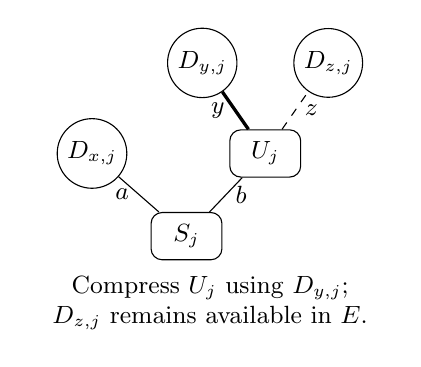
\begin{tikzpicture}[x=1cm,y=1cm,
 body/.style={draw,rounded corners,minimum width=9mm,minimum height=6mm},
 gropecap/.style={draw,circle,inner sep=2pt},
 every node/.style={font=\small}]
 \node[body] (s) at (0,0) {$S_j$};
 \node[gropecap] (a) at (-1.2,1.05) {$D_{x,j}$};
 \node[body] (u) at (1.0,1.05) {$U_j$};
 \node[gropecap] (y) at (0.2,2.2) {$D_{y,j}$};
 \node[gropecap] (z) at (1.8,2.2) {$D_{z,j}$};
 \draw (s)--node[left] {$a$}(a);
 \draw (s)--node[right] {$b$}(u);
 \draw[very thick] (u)--node[left] {$y$}(y);
 \draw[dashed] (u)--node[right] {$z$}(z);
 \node[align=center,text width=4.4cm] at (0.3,-0.85)
  {Compress \(U_j\) using \(D_{y,j}\);\\
   \(D_{z,j}\) remains available in \(E\).};
\end{tikzpicture}
\end{minipage}
\hfill
\begin{minipage}[c]{0.57\textwidth}
\centering
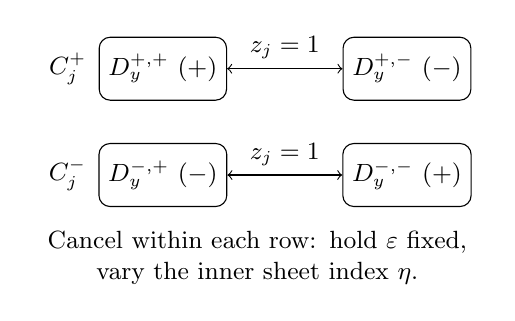
\begin{tikzpicture}[x=1cm,y=1cm,
 sheet/.style={draw,rounded corners,minimum width=1.45cm,minimum height=8mm},
 every node/.style={font=\small}]
 \node[sheet] (pp) at (0,1.1) {$D_y^{+,+}\ (+)$};
 \node[sheet] (pm) at (3.1,1.1) {$D_y^{+,-}\ (-)$};
 \node[sheet] (mp) at (0,-0.25) {$D_y^{-,+}\ (-)$};
 \node[sheet] (mm) at (3.1,-0.25) {$D_y^{-,-}\ (+)$};
 \draw[<->] (pp)--node[above] {$z_j=1$}(pm);
 \draw[<->] (mp)--node[above] {$z_j=1$}(mm);
 \node[anchor=east] at (-0.85,1.1) {$C_j^+$};
 \node[anchor=east] at (-0.85,-0.25) {$C_j^-$};
 \node[align=center,text width=5.6cm] at (1.2,-1.3)
  {Cancel within each row: hold \(\varepsilon\) fixed,\\
   vary the inner sheet index \(\eta\).};
\end{tikzpicture}
\end{minipage}
\caption{Combinatorial schematics, not projections of the four-dimensional
embedding. Left: the two-stage body and its one-sided upper contraction.
Right: the four occurrences of its surgery cap in the compressed rim
sphere; parentheses record their orientation coefficients
\(\varepsilon\eta\). The right panel suppresses the cap's subscript \(j\).
The labels \(z_j=1\) are equalities in \(\pi_1(E)\), proved using the upper
dual cap in \(E\).
No comparison between the two rows, which could involve a bottom
normal-circle meridian, is used.}
\label{fig:geometry-sheets}
\end{figure}


This accounts for every cap contribution to \(\lambda(f_i,g_j)\).
For \(g_i,g_j\), fix a sheet of \(g_i\) and the outer index of \(g_j\),
and cancel the inner index of \(g_j\) by the same argument. It also
applies when all parallel sheets at a plumbing point are counted
simultaneously. Hence the off-diagonal pairings of the \(g_j\) vanish.

The diagonal and framing admit a direct geometric check. The disk
\(C_j\) uses just the one core type \(D_{y,j}\), which has no self-plumbing.
That cap and its parallels are embedded and miss the parent body off their
attachments. Thus \(C_j\), and then the sphere in
\eqref{eq:compressed-rim-sphere}, can each be individually embedded.
Mutual intersections with other \(g_i\) do not affect this assertion.
The normal frame of the rim torus is
\((\partial_t,\partial_r)\). Along the outgoing radial compression collar
the cap normal frame is \((\partial_t,\partial_\theta)\).
Rounding the surgery corner rotates the second vector from
\(\partial_r\) to \(\partial_\theta\), while the first remains fixed.
The product framing matched in Lemma~\ref{lem:marked-body} extends this
ordered pair. The earlier compression \eqref{eq:one-sided-contraction}
is the same framed operation, so its outgoing \(b_j\)-annulus has exactly
the required inherited framing. Consequently \(g_j\) has trivial normal
bundle. Its normal push-off is disjoint from it, proving the diagonal
\(\lambda(g_j,g_j)=0\); its embedded representative also gives
\(\widetilde\mu(g_j)=0\).

Combining this with the distinguished collar point proves all the stated
equalities. Small perturbations make the finite collection generic while
preserving the calculation and the framings.
\end{proof}

Assumption~\ref{ass:disk}, applied to \(E\) and
Lemma~\ref{lem:exterior-duals}, now gives pairwise disjoint locally flat
embedded replacement caps with the specified boundary framings.
Compress each bottom \(S_j\) with two parallels of its replacement cap,
using the returning annuli in the removed tube. The result is a collection
of pairwise disjoint properly embedded disks in \(X\), bounded by the
initial grope boundaries. The framing is what makes this compression
locally flat with the required product collar. No relative homotopy of
the replacement cap to \(f_j\) is used. The output dual-sphere part of a
disk embedding theorem is not used either.

\subsection{Equivariant cuts with connected pieces}

The preceding compression uses the assumed replacement disks to make
the initial grope boundaries bound disjoint disks. We now keep those
disks in their prescribed vertex regions while cutting the ambient
plumbing into smooth pieces. Connectedness of these pieces will be
needed for the restriction maps in the final part of this section.

\begin{lemma}[Connected tree cuts]
\label{lem:connected-tree-cuts}
Suppose the initial grope boundaries bound the disjoint disks just
constructed. Then the boundary map to the plumbing tree extends
equivariantly to a map whose cuts can be chosen to have the connected
vertex and edge pieces asserted in
Proposition~\ref{prop:geometric-reduction}. Every lifted disk lies in
its prescribed vertex piece.
\end{lemma}

\begin{proof}
Lift the disks to \(\widetilde X\). Each is labelled by the vertex
containing its boundary. Distinct translates and distinct members have
disjoint images, because the disks were embedded and disjoint in \(X\).
Prescribe the map to be constant at the label vertex on a neighbourhood
of every such disk, and retain the fixed boundary map. These prescriptions
agree on their overlaps.

An equivariant extension is equivalently a section of the associated
bundle over \(X\) with fibre the tree. The prescribed section extends first
to a neighbourhood of the prescribed closed set, since the tree is an
absolute neighbourhood retract, and then over the remaining cells,
since the fibre is contractible. One may take a finite triangulation of
the smooth ambient manifold for the latter extension after shrinking the
neighbourhood. The section formulation ensures equivariance. This step
does not require extending to the noncontractible quotient graph by
contractibility of that graph.

On the quotient, approximate the map smoothly over the open middle
intervals of its finitely many graph edges, keeping it fixed on the
specified boundary collars and away from the disk neighbourhoods.
Choose regular values there. Their inverse images are compact smooth
proper hypersurfaces, disjoint from all disks. After rescaling an edge
interval we call its chosen value the midpoint. The lift of the level
corresponding to a tree edge \(e\) has exactly one boundary component:
the specified torus \(T_e\). More precisely, the unique component meeting
the boundary contains that torus as its entire boundary; every other
component of that level is closed.

Consider the component graph \(\mathcal T'\) of this cut in
\(\widetilde X\): its vertices are connected complementary pieces, and
its edges are connected cut hypersurfaces. It is connected. The collapse
to \(\mathcal T'\) is surjective on fundamental groups: a finite graph
loop is realised by choosing crossing points and joining successive
points by paths in the connected pieces. By
\eqref{eq:plumbing-homotopy}, the fundamental group of \(\widetilde X\)
is generated by the extra loops in its boundary pieces, with whiskers.
Each such loop maps to a vertex of \(\mathcal T'\). Thus
\(\pi_1\mathcal T'=0\), and \(\mathcal T'\) is a tree.

The boundary pieces and their torus collars determine a principal copy
\(\mathcal T\) of the original tree inside \(\mathcal T'\).
To check injectivity directly, remove the chosen midpoints from the
target tree. A connected component of their inverse-image complement
maps into just one resulting vertex-star component. It cannot contain
both \(K_v\) and \(K_w\) for \(v\ne w\). Similarly distinct principal
edge components have distinct midpoint labels. The boundary collars
give exactly the required incidences. Hence the principal copy is
indeed an embedded subtree.

Every remaining branch of \(\mathcal T'\) has a unique nearest vertex in
\(\mathcal T\). A deck transformation stabilising a vertex or edge of
such a branch fixes that nearest principal vertex and is therefore the
identity. Thus all these stabilisers are trivial. The finite compact
quotient cut has only finitely many components, so \(\mathcal T'\)
has finite quotient. Trivial stabilisers imply finite valence.
Moreover distance to \(\mathcal T\) is invariant under translation and
is bounded on the finite set of component orbits. A finite-valence tree
of bounded depth rooted at one principal vertex is finite.

Ignore the closed cuts in each such finite hanging branch, merging it
with its principal vertex piece. This operation is equivariant, preserves
compact quotient and the principal hypersurfaces, and gives connected
vertex pieces \(V_v\) and a single connected edge piece \(Y_e\) with
\(\partial Y_e=T_e\). All prescribed disks remain in their own pieces:
they lay in the component containing their boundary before the merging.
The \(Y_e\) and \(V_v\) are smooth manifolds with corners; the topological
disks themselves were never required to become smooth.
\end{proof}

Each initial boundary is therefore null-homotopic in its vertex piece.
Its actual boundary word has the three-slot properties
\eqref{eq:grope-word-properties} with inputs
\eqref{eq:three-slot-inputs}. This proves precisely the relation statement
in Proposition~\ref{prop:geometric-reduction}.

\subsection{The parity quotient and its peripheral homology}

Send every plumbing generator of \(F_m\) to \(1\in\mathbb Z/2\).
The quotient of \(\widetilde X\) by the kernel has two principal vertex
pieces \(A,B\) and two lifts of each of the \(m\) plumbing edges.
Thus there are \(2m\) edges. The free translation interchanging parity
gives a deck involution interchanging \(A\) and \(B\), and pairing these
edge lifts. Equation~\eqref{eq:plumbing-homotopy}, or the same
contractible-overlap argument in this quotient, gives
\begin{equation}
\label{eq:parity-homotopy}
 X_2\simeq\Gamma\ \text{with \(p\) extra circles at each vertex},
 \qquad
 |V\Gamma|=2,\quad |E\Gamma|=2m.
\end{equation}
In particular \(H^q(X_2;k)=0\) for \(q\geq2\), and
\(\dim_kH^1(X_2;k)=2m-1+2p\).
The extra loops at the two vertices can be assigned independently in
the free ambient fundamental group. All port meridians are trivial
there, since they bound the corresponding handle-core disks in \(X_2\).

\begin{lemma}[Restriction maps and coordinate slopes]
\label{lem:geometric-edge-cohomology}
The cohomology and slope conclusions of
Proposition~\ref{prop:geometric-reduction} hold.
For each edge piece one also has
\begin{equation}
\label{eq:edge-relative-cohomology}
 H^1(Y_i,\partial Y_i;k)
  \cong\ker\bigl(H^1(Y_i;k)\longrightarrow H^1(\partial Y_i;k)\bigr),
 \qquad b_2(Y_i)=b_1(Y_i)-1.
\end{equation}
\end{lemma}

\begin{proof}
Insert small edge collars so that Mayer--Vietoris applies to the two
vertex pieces with intersection the disjoint union of the \(Y_i\).
Its degree-one portion is
\[
\begin{aligned}
 H^0(A;k)\oplus H^0(B;k)
 &\longrightarrow\bigoplus_iH^0(Y_i;k)
 \longrightarrow H^1(X_2;k)\\
 &\longrightarrow H^1(A;k)\oplus H^1(B;k)
 \xrightarrow{\,R\,}\bigoplus_iH^1(Y_i;k)
 \longrightarrow0 .
\end{aligned}
\]
Connectedness makes the first cokernel have dimension \(2m-1\);
these are the graph classes of \(\Gamma\).
They restrict to zero on the vertex pieces. The remaining kernel of
\(R\) has dimension \(2p\). Evaluation on the \(p\) extra loops at each
vertex identifies this kernel with \(k^{2p}\): their ambient classes in
\eqref{eq:parity-homotopy} give surjectivity, and an ambient class with
zero extra evaluations is a graph class and restricts to zero.
Consequently \(R\) restricts to an isomorphism on the kernel of the
extra evaluations. The next part of the same sequence, using
\(H^2(X_2;k)=H^3(X_2;k)=0\), gives
\eqref{eq:geometry-mv-degree-two}.

Let \(Y\) be one of the connected oriented three-manifolds with single
torus boundary \(T\). Poincaré--Lefschetz duality and
\(\chi(Y)=\chi(T)/2=0\) give \(b_2(Y)=b_1(Y)-1\).
The exact sequence of the pair, using connectedness of \(Y,T\), gives
the isomorphism in \eqref{eq:edge-relative-cohomology}.
Equivalently the image of \(H_1(T;k)\) in \(H_1(Y;k)\) has dimension
one, the half-lives/half-dies statement.

Write \(u,v\) for the original two coordinate directions on \(T\).
One is a longitude in the boundary piece on one side and the other
is a longitude on the other side. Suppose both had nonzero image in
the one-dimensional image in \(H_1(Y;k)\). They would then be nonzero
scalar multiples of each other. A cohomology class restricted from
the first side annihilates its longitude and hence both directions;
the same is true of a class restricted from the second side.
Surjectivity of \(R\) would imply that every class of \(H^1(Y;k)\)
annihilates both directions, contradicting the one-dimensional image.
Thus one original coordinate direction has zero image and the other
has nonzero image. Denote them by \(\beta,\alpha\), respectively.
In cohomology the boundary restriction image is the line spanned by
the coordinate form dual to \(\alpha\).

The deck involution preserves the transported slope choice and swaps the
two vertices. For the two lifts of each plumbing edge it therefore
interchanges which one has its plus endpoint at \(A\).
Exactly one lift in each pair is active, giving exactly \(m\) active
edges. At \(A\) their \(\alpha\)'s are distinct port meridians, and at
\(B\) their \(\beta\)'s are distinct port meridians. Their three-slot
relations, with every independent choice of the stipulated conjugators,
were all included before any slope was selected.
\end{proof}

\begin{proof}[Proof of Proposition~\ref{prop:geometric-reduction}]
The plumbing construction supplies \(X\), its boundary pieces, and its
regular cover. Lemma~\ref{lem:marked-body} supplies the finite marked
family. Lemma~\ref{lem:exterior-duals} checks every input hypothesis of
Assumption~\ref{ass:disk} in the exterior of the bottoms.
The replacement disks and framed bottom compressions then give the
disks required by Lemma~\ref{lem:connected-tree-cuts}, and hence the
relations in connected vertex pieces. Finally
Lemma~\ref{lem:geometric-edge-cohomology} gives the claimed parity-quotient data.
\end{proof}
